%%%%%%%%%%%%%%%%%%%%%%%%%%%%%%%%%%%%%%%%%
%
% CMPT 333
% Lab 2
%
%%%%%%%%%%%%%%%%%%%%%%%%%%%%%%%%%%%%%%%%%

%%%%%%%%%%%%%%%%%%%%%%%%%%%%%%%%%%%%%%%%%
% LaTeX Template
% Version 1.0 (5/5/12)
%
% This template has been downloaded from: http://www.LaTeXTemplates.com
% Original author: % Frits Wenneker (http://www.howtotex.com)
% License: CC BY-NC-SA 3.0 (http://creativecommons.org/licenses/by-nc-sa/3.0/)
% Modified by Jason Gasparini
%
%%%%%%%%%%%%%%%%%%%%%%%%%%%%%%%%%%%%%%%%%

%----------------------------------------------------------------------------------------
%	PACKAGES AND OTHER DOCUMENT CONFIGURATIONS
%----------------------------------------------------------------------------------------

\documentclass[letterpaper, 10pt]{article} 

\usepackage[english]{babel} % English language/hyphenation
\usepackage{graphicx}
\usepackage[lined,linesnumbered,commentsnumbered]{algorithm2e}
\usepackage{listings}
\usepackage{fancyhdr} % Custom headers and footers
\pagestyle{fancyplain} % Makes all pages in the document conform to the custom headers and footers
\usepackage{lastpage}
\usepackage{url}

\fancyhead{} % No page header - if you want one, create it in the same way as the footers below
\fancyfoot[L]{} % Empty left footer
\fancyfoot[C]{page \thepage\ of \pageref{LastPage}} % Page numbering for center footer
\fancyfoot[R]{}

\renewcommand{\headrulewidth}{0pt} % Remove header underlines
\renewcommand{\footrulewidth}{0pt} % Remove footer underlines
\setlength{\headheight}{13.6pt} % Customize the height of the header

%----------------------------------------------------------------------------------------
%	TITLE SECTION
%----------------------------------------------------------------------------------------

\newcommand{\horrule}[1]{\rule{\linewidth}{#1}} % Create horizontal rule command with 1 argument of height

\title{	
   \normalfont \normalsize 
   \textsc{CMPT 333 - Fall 2023 } \\[10pt] % Header stuff.
   \horrule{0.5pt} \\[0.25cm] 	% Top horizontal rule
   \huge Lab 2 -- Reflection and Results \\     	    % Assignment title
   \horrule{0.5pt} \\[0.25cm] 	% Bottom horizontal rule
}

\author{Jason Gasparini \\ \normalsize Jason.Gasparini@Marist.edu}

\date{\normalsize\today} 	% Today's date.

\begin{document}

\maketitle % Print the title

%----------------------------------------------------------------------------------------
%   CONTENT SECTION
%----------------------------------------------------------------------------------------

% - -- -  - -- -  - -- -  -

\section{Reflection}
\vspace{1em}

\subsection{Erlang vs. Java}

With choosing to make use of the natural loops that are available to Java, coding this program between Erlang and Java required two different approaches. For a basic algorithm like this one, its complexity could be measured by how many total lines of code were needed. But, from my experience with this lab, that is not an accurate measurement of complexity. Because of the fact that I do not favor recursion over a basic for loop, the Erlang version was more complex yet it required many less lines to accomplish the same goal. The difficulty that I faced while coding the Erlang version can certainly be attributed to my inexperience with the syntax but also is because of the forced recursive nature. While this program in Erlang may be easier to code, I still think that it is harder to understand conceptually.

\vspace{2em}

\section{Results}

\begin{figure}
    \centering
    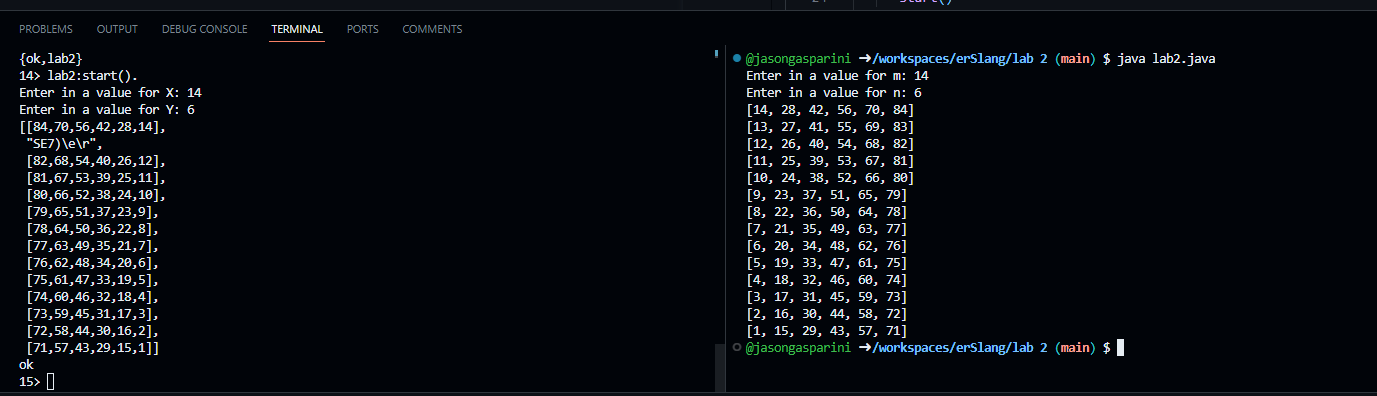
\includegraphics[width=\textwidth]{1.png}
    \caption{1st successful run mirrored across}
    \label{fig:1}
\end{figure}


\begin{figure}
    \centering
    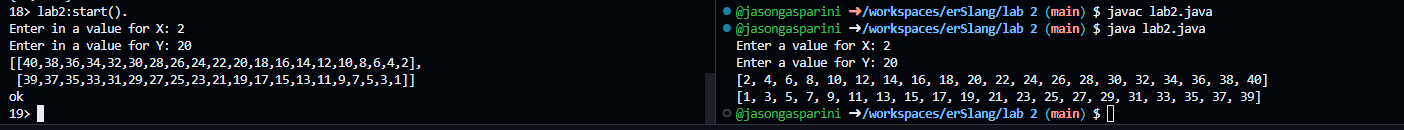
\includegraphics[width=\textwidth]{2.png}
    \caption{2nd successful run}
    \label{fig:2}
\end{figure}

\begin{figure}
    \centering
    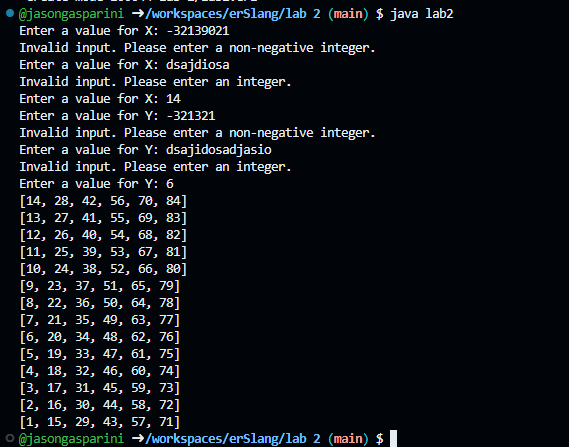
\includegraphics[width=\textwidth]{3.png}
    \caption{Java run with error checking/unexpected inputs}
    \label{fig:3}
\end{figure}

\begin{figure}
    \centering
    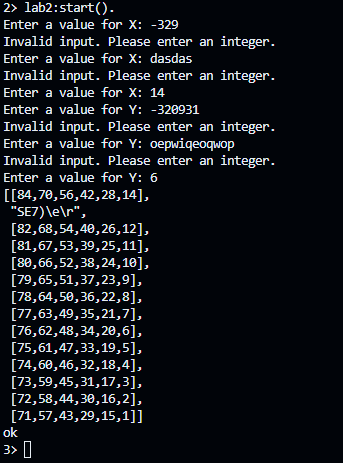
\includegraphics[width=\textwidth]{4.png}
    \caption{Erlang run with error checking/unexpected inputs, List 13 has all printable ASCII characters}
    \label{fig:4}
\end{figure}

\end{document}






